% \section{Deployment view: development and extensibility}
% \label{sec:Development}

The extensibility of LArSoft is largely based on the underlying
framework, \ART. The \ART framework processes physics event
independently, executing on each of them a sequence of modules.
The framework also provides a list of global ``services'' that modules can rely on.
Examples of services implemented by LArSoft include
the description of detector geometry and channel mapping,
the set of detector configuration parameters,
and access to TPC channel quality information.

In this section we describe the development environment
and then focus on the main handles LArSoft offers developers in terms of extensibility,
including new persistable data structures, new algorithms
and the use of external libraries.


\subsection{Development environment}
\label{ssec:Development:Environment}

LArSoft is designed for and supports the use of a development environment based on:
\begin{itemize}
   \item UNIX Product Support (\UPS) for access to dependent packages
   \item \cetbuildtools\cite{cetbuildtools} as build system
   \item Multi-Repository Build\cite{MRB} (\MRB)  to coordinate build and execute software from different repositories
   \item source code repositories under \git (recommended) or \SVN
\end{itemize}

LArSoft is fully supported on the following platforms:
\begin{itemize}
   \item Scientific Linux Fermi: version 6
   \item Darwin: version 13 (OS X 10.9 ``Maverick'') and 14 (OS X 10.10, ``Yosemite'')
\end{itemize}
LArSoft typically supports the two most recent versions of these operating systems\footnote{
The actual supported versions depend also on the underlying support of the O.S. by Fermilab.
}.
Support is also planned for the long term support release of Ubuntu Linux (16.04 LTS).

A typical workflow starts with the set up of a working area.
After the area is created, subsequent utilization of it requires just a simple set up.
LArSoft provides a script for this set up,
and it is common practise for the Experiments to provide customized ones.

The development, whether it is creation of new code or modification of existing one,
follows the following workflow:
\begin{enumerate}
   \item development-specific set up of the existing working area
   \item importing the source code to be modified, if any; this code will persist in the area
   \item modifications as needed
   \item building
   \item optional (and recommended) run of a standard test suite
   \item installation for running
\end{enumerate}

The execution of LArSoft code including user development, as described above,
follows this workflow:
\begin{enumerate}
   \item run-time specific set up of the existing working area
   \item execution of the software
\end{enumerate}
The execution of LArSoft code as distributed, without modification,
has a simpler set up that does not require a development working area.

LArSoft currently provides no facility to execute code remotely,
including job submission to remote clusters.
The Experiments supply workflows and scripts for this type of execution.



\subsection{Testing}
\label{ssec:Development:testing}

LArSoft development model allows multiple contributors to modify the
code at the same time. This model can create conflicts and dysfunction
in the code. Tests are instrumental to the early detection of such
defects. LArSoft includes tests at two levels, called \emph{unit tests}
and \emph{integration tests}.

Unit tests exercise a limited part of the system, typically a single
algorithm. Ideally a unit test for an algorithm should test all the
functions of that algorithm. In practice, tests for complex algorithms
tend to set up and test a few known typical cases.

Integration tests involve the framework and one or more processing
modules. These tests can reproduce real user scenarios, for example a
part of the official processing chain of an experiment, and they can
compare new and historical results. LArSoft tools allow these tests to
be run at any time, and a standard suite of tests is meant to be
automatically and periodically run.



\subsection{Data products}
\label{ssec:Development:DataProducts}

LArSoft provides a basic set of persistable data classes.
Each class is associated to a simple concept and a set of related quantities.
For example, \texttt{raw::RawDigit} describes the raw data as read from a TPC channel;
\texttt{recob::Cluster} describes a set of hits observed on a wire plane;
\texttt{anab::Calorimetry} contains information about calibrated energy of a track.

A \emph{data product} is a class that:
\begin{itemize}
   \item is simple: contains just data and trivial logic to access it;
      more complex elaborations belong to algorithms
   \item contains only members from a small selected libraries:
      C++ standard library is highly recommended; ROOT classes are also accepted
   \item is not polymorphic
\end{itemize}

Limitations to ROOT I/O system impose restrictions on the types of allowed data members,
\eg on the set of supported C++11 containers.
Relations between data products are expressed by \emph{associations}.
Associations are data products provided by \emph{art}
which can relate a data product, or an element of it,
to another element from another data product.
Examples of use in LArSoft include associations between a
reconstructed hit and the calibrated signal it's reconstructed from, and
between a cluster and all the hits that constitute it.

Data products have a fundamental structural role:
they act as messages to be exchanged between algorithms.
As such, they are also the format in which most of the results are saved.
This allows to arbitrary split the processing chain in multiple sequences of jobs.


\subsection{User code}
\label{ssec:Development:UserCode}

Algorithms constitute, together with data products, the heart of LArSoft,
and the ability for user to add their own algorithm is central to its design.
In fact, LArSoft algorithms differ from users' algorithms
only in the judgment that their purpose is considered of wider interest
than just for the single user.
Indeed, most of the algorithms in LArSoft were written by users to solve their own specific problems,
and then adopted into the common toolkit.
LArSoft encourages users to produce algorithms that perform correctly on \emph{any} liquid argon detector,
and to integrate them into LArSoft itself.

\begin{figure}
   \centering
   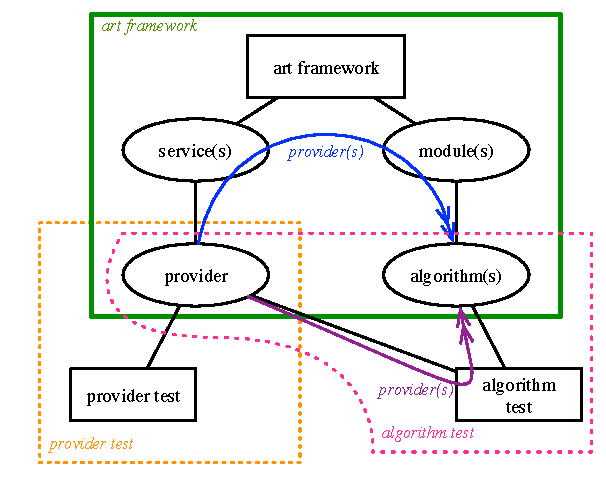
\includegraphics{figures/LArSoftFactorizationModelAndTests.pdf}
   \caption{\label{fig:AlgorithmModel}LArSoft algorithm and service model.
      Black lines represent ownership.
      The coloured lines show the path the algorithm obtains the provider through.
      Both service providers and algorithms can be tested without involving the full framework.
   }
\end{figure}

The preferred model for algorithm structure is represented in \cref{fig:AlgorithmModel}.
We refer to this as \emph{factorization} model.
The underlying principle it is that the algorithm must be independently
testable and portable, using the minimal set of necessary dependences.
This also allows for the algorithms to be used in contexts where the
\ART framework is not available,
provided that some other system supplies equivalent functionalities as,
and only when, needed. The model is made of two layers:
\begin{enumerate}
   \item
      the algorithm, in the form of a class that
      \begin{itemize}
         \item
            is configurable with FHiCL parameter sets
         \item
            consumes LArSoft data products as input
         \item
            produces LArSoft data products as output
         \item
            has the minimal convenient set of dependencies
         \item
            elaborates a single event or part of an event at a time
      \end{itemize}
   \item
      a module for the \ART framework, that:
      \begin{itemize}
         \item
           owns and manages the lifetime of one or more algorithm classes
         \item
           provides the algorithm(s) with the configuration, the data products
           and the information it needs to operate
         \item
           delivers algorithm output to the \ART framework
      \end{itemize}
\end{enumerate}

Since algorithms often rely on services, the services also need to
follow the same factorization model and be split in:

\begin{enumerate}
   \item
      a \emph{service provider}, in the form of a class that:
      \begin{itemize}
         \item
            is configurable with FHiCL parameter sets
         \item
            has the minimal convenient set of dependencies
         \item
            provides the actual functionalities
      \end{itemize}
   \item
      a service for the \emph{art} framework, that:
      \begin{itemize}
         \item
            owns and manages the lifetime of its service provider
         \item
            provides modules with a pointer to the provider
         \item
            when relevant, propagates messages from the framework (e.g., the
            beginning of a new run) to the provider
      \end{itemize}
\end{enumerate}
The module is also responsible of communicating to its algorithms which
service providers to use. Algorithms exclusively interact with service
providers rather than with \ART services.

Other important guidelines for the development of algorithms are:

\begin{description}
   \item[interoperability]
      they should document their assumptions in detail,
     and correctly perform on any detector if possible
   \item[modularity]
      each algorithm should perform a single task;
      complex tasks can be performed by hierarchies of algorithms
   \item[maintainability]
      they should come with complete documentation and proper tests
\end{description}

\Cref{fig:AlgorithmModel} shows that if algorithms are not
framework-dependent, their unit test can also be framework-independent.
Therefore, not only those algorithms can be developed in a simplified,
framework-unaware environment, but they can also be tested in that same
development environment. In other words, the full development cycle, of
which testing is an integral part, can seamlessly happen in the same
environment.

\subsection{External libraries}\label{external-libraries}

We call ``external'' any library that does not depend on LArSoft, with
the possible exception of its data products. Examples in this category
are \GENIE, \GEANT, and \Pandora.

\begin{figure}[htbp]
\centering

\includegraphics[width=\textwidth]{figures/LArSoftAndExternals.pdf}
\caption{\label{fig:LArSoftAndExternals}Interaction between LArSoft and
an external library}
\end{figure}

LArSoft's modularity can accommodate contributions from external
libraries into its workflow (\cref{fig:LArSoftAndExternals}). The
preferred way is to use directly the external library via its interface.
This requires an additional interface module between LArSoft and the
library, in charge of converting the LArSoft data products into a format
digestible by the external library, configuring and driving it, and
extracting and converting the results into a set of LArSoft data
products.

\begin{figure}[htbp]
\centering
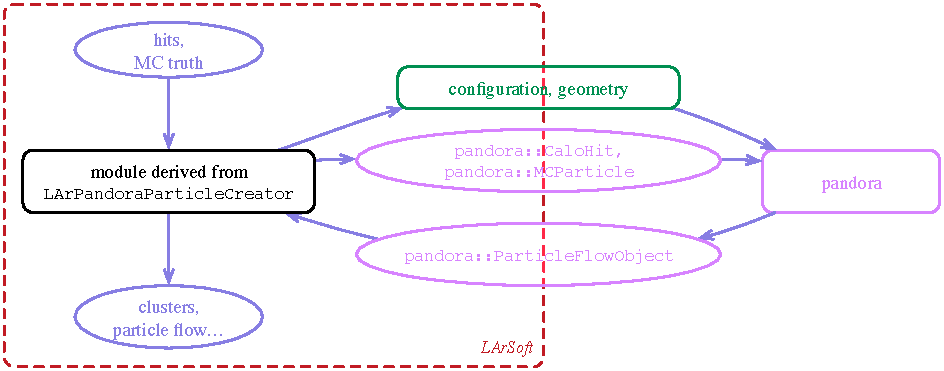
\includegraphics[width=\textwidth]{figures/LArSoftAndPandora.pdf}
\caption{\label{fig:LArSoftAndPandora}Interaction between LArSoft and
\Pandora}
\end{figure}

This is exemplified in the interaction between LArSoft and
\Pandora (\cref{fig:LArSoftAndPandora}): \Pandora uses
its own data classes for input hits, particle flow results and geometry
specification. A base module exists that reads LArSoft hits, converts
them into \Pandora's, translates geometry information, and
recreates out of \Pandora particle flow objects LArSoft clusters,
tracks, vertices, and more.

This approach has relevant advantages: it can be fairly fast; it allows
a precise translation of information; it provides the greatest control
on the flow within the library; it defines and tracks the configuration
of the external library. Its greatest drawback is the need for the
LArSoft interface to depend on the external library. If this limitation
is not acceptable, a more independent communication channel can be
established via exchange files. In this case, LArSoft interface
translates data products into a neutral format, possibly based solely on
ROOT objects or on a textual representation, and back into data
products. The external library is in charge of performing the equivalent
operations with the library data format. This is for example the generic
communication mechanism with event generators that support HEPEVT
format. The strong decoupling comes at the price of a fragmented
execution chain and the burden of additional configuration consistency
control, for example to ensure that a consistent geometry was used for
the information (re)entering LArSoft.
